\documentclass[12pt,a4paper]{article}
\usepackage[utf8]{inputenc}
\usepackage[T1]{fontenc}
\usepackage{babel}
\babelprovide[import,main]{spanish}
\usepackage{lmodern,microtype}
\usepackage[margin=2.5cm,headheight=15pt]{geometry}
\usepackage{booktabs,longtable,array,enumitem,xcolor,titlesec,fancyhdr,lastpage}
\usepackage{tikz,needspace,placeins}
\usetikzlibrary{arrows.meta,positioning}
\PassOptionsToPackage{obeyspaces}{url}
\usepackage{hyperref}
\definecolor{sectionblue}{RGB}{31,78,121}
\hypersetup{colorlinks=true,linkcolor=sectionblue,urlcolor=sectionblue,citecolor=sectionblue,
 pdftitle={Reimplementación compatible de OpenStack Glance: Etapa 2},pdfauthor={Juan Cardenas Uribe}}
\titleformat{\section}{\Large\bfseries\color{sectionblue}}{\thesection}{0.8em}{}
\titleformat{\subsection}{\normalsize\bfseries}{\thesubsection}{0.8em}{}
\titlespacing*{\section}{0pt}{16pt}{9pt}
\titlespacing*{\subsection}{0pt}{12pt}{6pt}
\setlength{\parindent}{0pt}
\setlength{\parskip}{6pt}
\setcounter{tocdepth}{2}
\emergencystretch=2em
\raggedbottom
\clubpenalty=10000
\widowpenalty=10000
\setlist{nosep,topsep=5pt,leftmargin=*}
\renewcommand{\tablename}{Cuadro}
\addto\captionsspanish{\renewcommand{\tablename}{Cuadro}}
\pagestyle{fancy}
\fancyhf{}
\fancyhead[L]{\small Trabajo de Título -- Etapa 2}
\fancyhead[R]{\small INFO-1197}
\fancyfoot[C]{\small\thepage\ de \pageref{LastPage}}
\renewcommand{\headrulewidth}{0.4pt}
\renewcommand{\footrulewidth}{0pt}
\newcommand{\code}[1]{{\small\expandafter\nolinkurl\expandafter{\detokenize{#1}}}}
\newcommand{\reporttable}[4]{\begingroup\small\setlength{\LTpre}{8pt}\setlength{\LTpost}{8pt}\setlength{\tabcolsep}{4pt}\renewcommand{\arraystretch}{1.15}
\begin{longtable}{#2}\caption{#1}\\\toprule #3\\\midrule\endfirsthead
\toprule #3\\\midrule\endhead\bottomrule\endfoot #4\end{longtable}\endgroup}
\newcommand{\reportcover}{
\hypersetup{pageanchor=false}
\begin{titlepage}\centering
\vspace*{0.3cm}
{\Large Universidad Católica de Temuco\par}
\vspace{0.2cm}{\large Ingeniería Civil en Informática\par}
\vspace{2cm}
{\LARGE\bfseries Reimplementación compatible de\\OpenStack Glance\\en un lenguaje compilado\par}
\vspace{0.65cm}
{\large\bfseries Etapa 2: análisis, diseño y línea base\par}
\vspace{1.8cm}
\begin{tabular}{rl}
\textbf{Estudiante:}&Juan Cardenas Uribe\\[0.35cm]
\textbf{Profesor guía:}&Alejandro Mellado Gatica\\[0.35cm]
\textbf{Curso:}&Trabajo de Título (INFO-1197)\\[0.35cm]
\textbf{Fecha:}&2 de octubre de 2026
\end{tabular}
\vfill Temuco, Chile
\end{titlepage}
\pagenumbering{arabic}\hypersetup{pageanchor=true}\begingroup\small\setlength{\parskip}{0pt}\tableofcontents\endgroup\newpage}
\begin{document}
\reportcover

\section{Introducción}
OpenStack Glance permite registrar, consultar y distribuir imágenes utilizadas para crear instancias. El servicio combina un catálogo de metadatos con almacenamiento de archivos binarios y acceso autenticado. Esa combinación permite estudiar una reimplementación que debe preservar tanto la API como la integridad de los datos \cite{glanceoverview,glanceapi}.

Este informe corresponde al trabajo de Juan Cardenas Uribe y concentra el análisis en Glance. Conserva la organización del documento de Etapa 1: definición del problema, objetivos, requerimientos, planificación y conclusiones. En la Etapa 2 se agregan arquitectura, contrato Image API, persistencia, flujo de datos y evidencia de la línea base.

Se propone Go para una implementación acotada de Image API v2. La evaluación posterior deberá comparar compatibilidad, latencia, throughput y recursos. No se supone una mejora automática por el cambio de lenguaje. Esta etapa verifica el servicio original y define el diseño; aún no existe una implementación Go aceptada ni benchmarks comparativos.

El laboratorio es común con el trabajo de Placement. Ese servicio permanece como dependencia original al evaluar Glance. Los resultados de instalación y smoke tests se presentan como evidencia compartida, sin atribuir su ejecución exclusivamente al autor de este informe.

\section{Definición del problema}
\subsection{Contexto}
Nova necesita información y datos de imagen para crear una instancia. Glance expone Image API v2, aplica autenticación y políticas, conserva metadatos en una base de datos y delega el almacenamiento binario en un backend. Metadatos y bytes deben mantenerse coherentes a través del ciclo de vida de la imagen \cite{glanceapi,glanceoverview}.

La línea base proviene de DevStack de un nodo, con un único backend filesystem. Permite probar registro, actualización, transferencia, eliminación e integración con Nova, sin introducir la complejidad de almacenamiento distribuido.

\subsection{Problema identificado}
Una reimplementación que almacena registros de imagen pero altera estados, formatos, políticas o bytes puede responder a la API y aun así impedir el boot de una instancia. La transferencia de imágenes también puede consumir memoria de forma distinta según el diseño. El problema es conservar un ciclo mínimo compatible y evaluar su costo bajo condiciones controladas.

La pregunta de investigación es: \textit{¿es posible reimplementar el alcance seleccionado de Glance en Go, manteniendo la gestión de imágenes y su consumo por Nova, y qué diferencias de rendimiento y recursos presenta frente al servicio original?}

\subsection{Relevancia e impacto}
El resultado esperado incluye un contrato reproducible de Image API v2 y un prototipo que integre metadatos, persistencia y transferencia binaria. La investigación podrá distinguir los costos de procesamiento de metadatos de los costos de transferencia y almacenamiento. Las conclusiones deberán reportar mejoras, regresiones y límites del backend seleccionado.

\subsection{Partes interesadas y percepción del problema}
\reporttable{Partes interesadas del proyecto Glance.}{>{\raggedright\arraybackslash}p{3.6cm}>{\raggedright\arraybackslash}p{11.4cm}}{\textbf{Parte interesada}&\textbf{Necesidad o interés}}{
Estudiante responsable&Juan Cardenas Uribe: delimitar, diseñar e implementar Glance y sustentar su evaluación.\\*
Profesor guía&Validar la coherencia entre alcance, resultados y evidencia del trabajo de título.\\*
Usuarios y clientes API&Gestionar imágenes con respuestas, estados y reglas compatibles.\\*
Nova&Consumir metadatos y datos de imagen para el escenario de boot comprometido.\\*
Equipo del laboratorio&Repetir instalación y pruebas; aislar la sustitución de Glance.\\}

\subsection{Alcance y límites}
El alcance incluye crear, listar, consultar, actualizar y eliminar metadatos; cargar y descargar datos binarios; conservar autenticación requerida por el laboratorio; y permitir que Nova cree una instancia desde una imagen servida por el reemplazo.

Se utiliza un único backend de archivos local. Multi-store, importación interoperable completa, replicación, federación, caché distribuida y metadefs completos quedan fuera del alcance inicial, salvo que una prueba de integración demuestre una dependencia necesaria. Se deben definir límites de formato, visibilidad y permisos a partir de los casos comprometidos.

El original anunció Image API v2.18. Esa versión describe la API de Glance y no se trata como la negociación de microversiones de Placement. Keystone, Nova, Placement, Neutron y la virtualización permanecen como componentes originales. La evaluación no representa producción ni escalado multinodo.

\Needspace{165pt}
\section{Objetivos}
\subsection{Objetivo general}
Diseñar, implementar y evaluar una reimplementación compatible del subconjunto seleccionado de OpenStack Glance en Go, que permita gestionar y transferir imágenes e integrarse con Nova, comparando su funcionamiento, rendimiento y recursos con el servicio original.

\subsection{Objetivos específicos}
Los identificadores OE1--OE5 mantienen la trazabilidad de la planificación común; la aplicación de cada objetivo se concentra aquí en Glance. El hito de 50\% de implementación corresponde al proyecto conjunto; el Excel ubica las historias B20 y B25 de Glance en Sprint 4.
\begin{enumerate}[label=\textbf{OE\arabic*.}]
\item Analizar arquitectura, Image API, autenticación, persistencia y flujo de datos antes del 2 de octubre de 2026.
\item Disponer del laboratorio reproducible y verificar la línea base del ciclo de imagen y el boot original antes del 2 de octubre de 2026.
\item Contribuir al hito común de al menos 50\% de implementación del proyecto al 30 de octubre de 2026, preparando el esqueleto y fixtures de Glance para las historias de Sprint 4.
\item Integrar y estabilizar gestión de metadatos y transferencia binaria antes del 20 de noviembre de 2026, preparando la sustitución con Nova prevista por B26 en S5.
\item Validar el boot con Glance Go (B26), comparar compatibilidad, latencia, throughput, CPU, memoria y errores, y presentar conclusiones antes del 4 de diciembre de 2026.
\end{enumerate}

\subsection{Verificación SMART}
\reporttable{Objetivos Glance, indicadores y estado al cierre de Sprint 2.}{>{\raggedright\arraybackslash}p{1cm}>{\raggedright\arraybackslash}p{8cm}>{\raggedright\arraybackslash}p{2.5cm}>{\raggedright\arraybackslash}p{2.8cm}}{\textbf{ID}&\textbf{Indicador y evidencia}&\textbf{Plazo}&\textbf{Estado}}{
OE1&Arquitectura, endpoints, datos, estados, backend y flujo de integración documentados.&02-10-2026&Cumplido en S2.\\*
OE2&Ciclo original probado, descarga idéntica, rechazo sin token y boot ACTIVE.&02-10-2026&Cumplido en S2.\\*
OE3&Hito común: 50\% del proyecto; Glance prepara esqueleto y fixtures para su implementación.&30-10-2026&Planificado.\\*
OE4&Catálogo y transferencia estabilizados; boot del reemplazo B26 queda programado en S5.&20-11-2026&Planificado.\\*
OE5&Dataset de metadata/transferencia, repeticiones y análisis comparativo.&04-12-2026&Planificado.\\}
El cumplimiento de OE1 se limita a la especificación de Sprint 2. No implica haber verificado cada política, error o estado de la API completa; esos casos se ampliarán durante el desarrollo.

\Needspace{220pt}
\subsection{Matriz de trazabilidad problema--objetivos}
\reporttable{Trazabilidad del problema Glance.}{>{\raggedright\arraybackslash}p{4.4cm}>{\raggedright\arraybackslash}p{1.8cm}>{\raggedright\arraybackslash}p{8.7cm}}{\textbf{Aspecto del problema}&\textbf{Objetivo}&\textbf{Resultado verificable}}{
Contrato, estados y almacenamiento&OE1&Inventario Image API, modelo y separación metadata/bytes.\\*
Pruebas difíciles de repetir&OE2&Laboratorio automatizado y ciclo de imagen original documentado.\\*
Integridad y consumo por Nova&OE3/OE4&Transferencia idéntica, persistencia y boot con Glance Go.\\*
Eficiencia sin evidencia&OE5&Mediciones separadas de operaciones metadata y transferencia.\\}

\section{Análisis de requerimientos}
\subsection{Base técnica y arquitectura del servicio}
El servicio desplegado separa API HTTP, autenticación/políticas, controladores y dominio, persistencia de metadatos y \code{glance_store}. Los archivos de configuración y las tablas reales se contrastaron con los modelos del código fijado. El backend confirmado usa \code{/opt/stack/data/glance/images/} \cite{repo}.

\begin{figure}[ht]
\centering
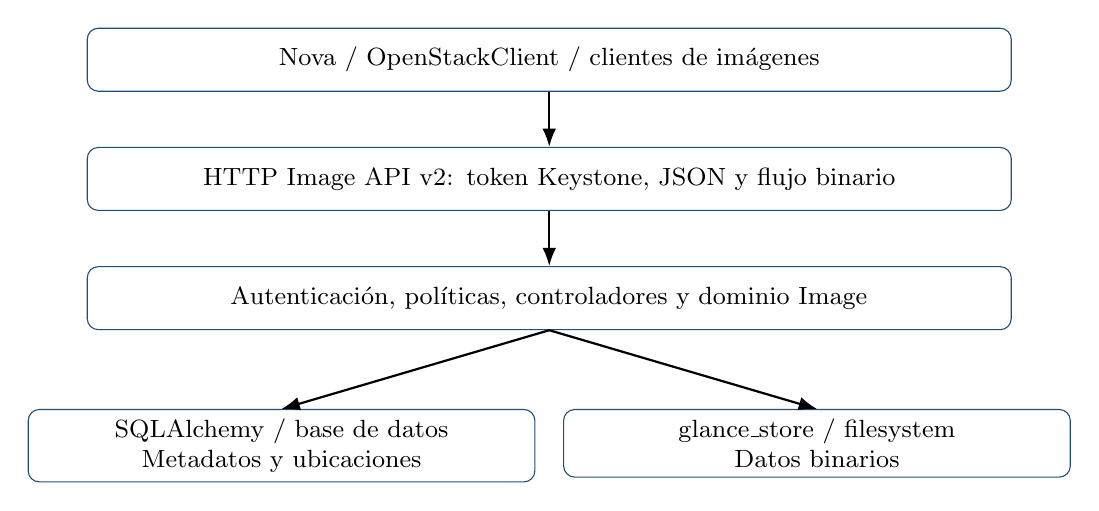
\begin{tikzpicture}[node distance=0.7cm,box/.style={draw=sectionblue,rounded corners,align=center,text width=11.5cm,minimum height=0.8cm,font=\small},smallbox/.style={box,text width=6.2cm},arr/.style={-{Latex},thick}]
\node[box](client){Nova / OpenStackClient / clientes de imágenes};
\node[box,below=of client](api){HTTP Image API v2: token Keystone, JSON y flujo binario};
\node[box,below=of api](domain){Autenticación, políticas, controladores y dominio Image};
\node[smallbox,below=1cm of domain,xshift=-3.4cm](db){SQLAlchemy / base de datos\\Metadatos y ubicaciones};
\node[smallbox,below=1cm of domain,xshift=3.4cm](store){glance\_store / filesystem\\Datos binarios};
\draw[arr](client)--(api);\draw[arr](api)--(domain);\draw[arr](domain.south)--(db.north);\draw[arr](domain.south)--(store.north);
\end{tikzpicture}
\caption{Separación de metadatos y datos de imagen en el servicio original.}
\end{figure}

\subsection{Selección del servicio y del lenguaje}
Glance aporta un caso de investigación que combina llamadas de metadatos, persistencia y transferencia de archivos. Un alcance limitado a Image API v2 y filesystem permite evaluar esa combinación sin implementar todos los backends de OpenStack.

Go se selecciona por su soporte HTTP y de concurrencia, compilación a binario y facilidad para organizar adaptadores de almacenamiento. El beneficio de streaming sobre memoria o throughput debe verificarse; no se atribuye automáticamente al lenguaje.
\reporttable{Alternativas de lenguaje para Glance.}{>{\raggedright\arraybackslash}p{4.3cm}>{\raggedright\arraybackslash}p{3.2cm}>{\raggedright\arraybackslash}p{3.2cm}>{\raggedright\arraybackslash}p{3.6cm}}{\textbf{Criterio}&\textbf{Go}&\textbf{Rust}&\textbf{C++}}{
API y transferencia&HTTP e interfaces de streaming disponibles.&Buen soporte; mayor curva inicial.&Requiere integrar bibliotecas.\\*
Memoria y concurrencia&Gestión automática y goroutines.&Propiedad y seguridad estática.&Control manual más complejo.\\*
Riesgo en el plazo&Moderado.&Mayor costo inicial estimado.&Mayor costo de integración estimado.\\*
Decisión&Seleccionado.&Alternativa.&No priorizado.\\}
La comparación expresa la valoración de diseño del proyecto, no una medición experimental de rendimiento entre lenguajes.

\subsection{Entorno de despliegue: DevStack versus instalación manual}
Se utiliza DevStack para automatizar instalación y configuración en un laboratorio de desarrollo \cite{devstack}. Una instalación manual ofrecería más control por componente, con mayor tiempo y documentación de configuración. Terraform y Ansible hacen repetible la alternativa elegida.

La VM compartida \code{tt-openstack-lab} tiene Ubuntu 24.04.5, 4 vCPU, 8 GiB de RAM y disco de 55 GiB. Se verificaron Keystone, Nova, Placement, Glance, Neutron, MySQL y RabbitMQ. El smoke test utiliza QEMU emulado; una segunda ejecución de Ansible terminó sin reinstalar DevStack.
\reporttable{Versiones registradas en la línea base Glance.}{>{\raggedright\arraybackslash}p{4cm}>{\raggedright\arraybackslash}p{11cm}}{\textbf{Componente}&\textbf{Versión o commit}}{
DevStack&\code{stable/2026.2}; \code{0fb9685c1bf22cd0b4d576d7a74f64195ad934fe}.\\*
Glance&\code{a3e5f490b7a28b1161714c94acffe5308d24b567}.\\*
Nova&\code{247ea5d774305b688997f8df81c011b249eb793c}.\\*
Python / MySQL&3.12.3 / 8.0.46.\\*
Image API / OpenStackClient&v2.18 anunciada / 10.3.0.\\}
La configuración y un parche Geneve están versionados. Las dependencias secundarias no se fijaron para una reconstrucción bit a bit. La VM quedó apagada por solicitud del usuario después de registrar la evidencia, conservando sus discos; no se ejecutaron pruebas nuevas para elaborar este documento.

\subsection{Contrato Image API v2}
La API utiliza tokens Keystone. Metadata usa JSON; la carga binaria emplea \code{application/octet-stream}; PATCH utiliza \code{application/openstack-images-v2.1-json-patch}. Los resultados de la línea base original se detallan a continuación.
\reporttable{Operaciones Glance y resultados de la línea base.}{>{\raggedright\arraybackslash}p{6.8cm}>{\raggedright\arraybackslash}p{1.5cm}>{\raggedright\arraybackslash}p{6.7cm}}{\textbf{Método y ruta}&\textbf{HTTP}&\textbf{Resultado observado}}{
\texttt{\small POST}\,\code{/v2/images}&201&Imagen registrada en estado queued.\\*
\texttt{\small GET}\,\code{/v2/images}&200&Listado de imágenes autenticado.\\*
\texttt{\small GET}\,\code{/v2/images/{id}}&200&Consulta de metadatos y estado.\\*
\texttt{\small PATCH}\,\code{/v2/images/{id}}&200&Actualización de metadatos mediante JSON Patch.\\*
\texttt{\small PUT}\,\code{/v2/images/{id}/file}&204&Carga de bytes; consulta posterior en active.\\*
\texttt{\small GET}\,\code{/v2/images/{id}/file}&200&Descarga idéntica byte a byte y por SHA256.\\*
\texttt{\small DELETE}\,\code{/v2/images/{id}}&204&Eliminación del recurso temporal.\\*
\texttt{\small GET}\,\code{/v2/images/{id}} ausente&404&Recurso inexistente tras eliminación.\\*
\texttt{\small GET}\,\code{/v2/images} sin token&401&Rechazo de la petición no autenticada.\\}
Las políticas de visibilidad, propietario y roles necesitan fixtures específicos de 403 y acceso permitido. También faltan casos de PATCH inválido, transferencia interrumpida, límites de tamaño y conflicto. El éxito del camino principal no acepta automáticamente estos comportamientos del reemplazo.

\subsection{Modelo de datos y ciclo de vida}
Los metadatos de \code{images} incluyen UUID, nombre, propietario, estado, visibilidad, formatos, tamaño, checksum, hashes, mínimos de disco/RAM, protección y timestamps. Los bytes se almacenan fuera de la base de datos. La auditoría confirmó las tablas; el detalle de claves proviene de los modelos SQLAlchemy fijados.
\reporttable{Entidades y almacenamiento del dominio Glance.}{>{\raggedright\arraybackslash}p{3.6cm}>{\raggedright\arraybackslash}p{6.2cm}>{\raggedright\arraybackslash}p{5.2cm}}{\textbf{Entidad}&\textbf{Datos centrales}&\textbf{Regla de diseño}}{
Image&UUID PK, propietario, estado, formatos, tamaño y hashes.&Identidad y ciclo de vida consistentes.\\*
ImageProperty&ID, image\_id, nombre y valor; unicidad imagen/nombre.&Actualizar propiedades con validación.\\*
ImageLocation&ID, image\_id, ubicación, metadata y estado.&Relacionar ubicación con el backend autorizado.\\*
ImageTag / ImageMember&Etiquetas y membresía de acceso.&Delimitar operaciones según los casos necesarios.\\*
Store filesystem&Archivo binario separado del catálogo.&Integridad, permisos y limpieza de datos.\\}
Se observó queued tras crear la imagen y active después de cargar los datos. Saving y killed forman parte del análisis del ciclo de carga, pero no se observaron en pruebas de fallo de esta etapa; deben comprobarse antes de aceptar recuperación de errores.

Se propone un esquema propio acotado para metadatos y un adaptador filesystem. El diseño escribe a un archivo temporal, calcula tamaño/hash y publica mediante rename atómico antes de confirmar active. Como base de datos y filesystem no comparten una transacción, se necesita reconciliación y limpieza ante fallos. Esa recuperación es una tarea de implementación y prueba, no una propiedad ya demostrada.


\Needspace{275pt}
\begin{figure}[!ht]
\centering
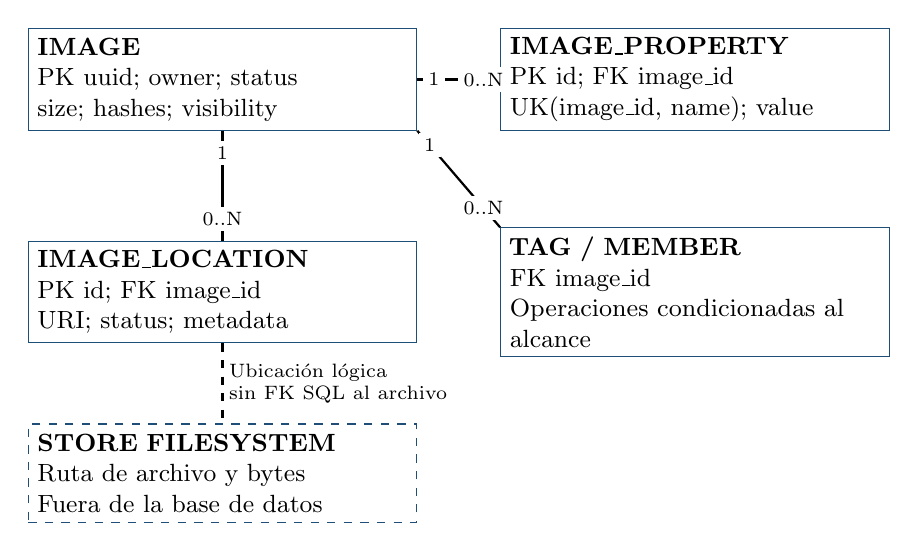
\begin{tikzpicture}[ent/.style={draw=sectionblue,align=left,text width=4.7cm,minimum height=1.25cm,font=\small},rel/.style={thick},lab/.style={font=\scriptsize,fill=white,inner sep=2pt}]
\node[ent](image) at (0,0){\textbf{IMAGE}\\PK uuid; owner; status\\size; hashes; visibility};
\node[ent](props) at (6,0){\textbf{IMAGE\_PROPERTY}\\PK id; FK image\_id\\UK(image\_id, name); value};
\node[ent](loc) at (0,-2.7){\textbf{IMAGE\_LOCATION}\\PK id; FK image\_id\\URI; status; metadata};
\node[ent](tags) at (6,-2.7){\textbf{TAG / MEMBER}\\FK image\_id\\Operaciones condicionadas al alcance};
\node[ent,dashed](file) at (0,-5){\textbf{STORE FILESYSTEM}\\Ruta de archivo y bytes\\Fuera de la base de datos};
\draw[rel](image)--node[lab,pos=0.2]{1}node[lab,pos=0.8]{0..N}(props);
\draw[rel](image)--node[lab,pos=0.2]{1}node[lab,pos=0.8]{0..N}(loc);
\draw[rel](image.south east)--node[lab,pos=0.15]{1}node[lab,pos=0.8]{0..N}(tags.north west);
\draw[rel,dashed](loc)--node[lab,right,align=left]{Ubicación lógica\\sin FK SQL al archivo}(file);
\end{tikzpicture}
\caption{Modelo ER del catálogo Glance y relación externa con el store. PK, FK y UK identifican claves del modelo original; el esquema Go es propio.}
\label{fig:er}
\end{figure}
\FloatBarrier
La figura \ref{fig:er} separa datos relacionales y binarios. La estrategia Go debe recuperar una publicación interrumpida: limpiar temporales incompletos y reconciliar archivos finales sin metadata confirmada. El tamaño/hash y el estado de imagen se verifican conjuntamente en RF07/RF10. No se supone atomicidad distribuida entre SQL y filesystem.

\subsection{Flujo de datos e integración con Nova}
El flujo mínimo verificado fue registro de imagen, carga de bytes, consulta, modificación de metadata, descarga, comparación y eliminación. El baseline preservó requests, respuestas, status y headers saneados. La igualdad de bytes y SHA256 sustenta la integridad del caso original probado.

El smoke test creó una instancia desde CirrOS y registró la transición BUILD a ACTIVE. La instancia fue eliminada después de la verificación. Este resultado comprueba la integración general del OpenStack original, pero no captura la conversación HTTP interna Nova--Glance ni permite afirmar qué descarga o uso de caché ejecutó Nova.

Para aceptar el reemplazo, Nova deberá consultar y consumir una imagen gestionada por Go. Se capturará el flujo real y se controlará el estado de caché de la prueba. Placement permanecerá original en ese escenario para aislar las diferencias del módulo Glance.


\Needspace{310pt}
\begin{figure}[!ht]
\centering
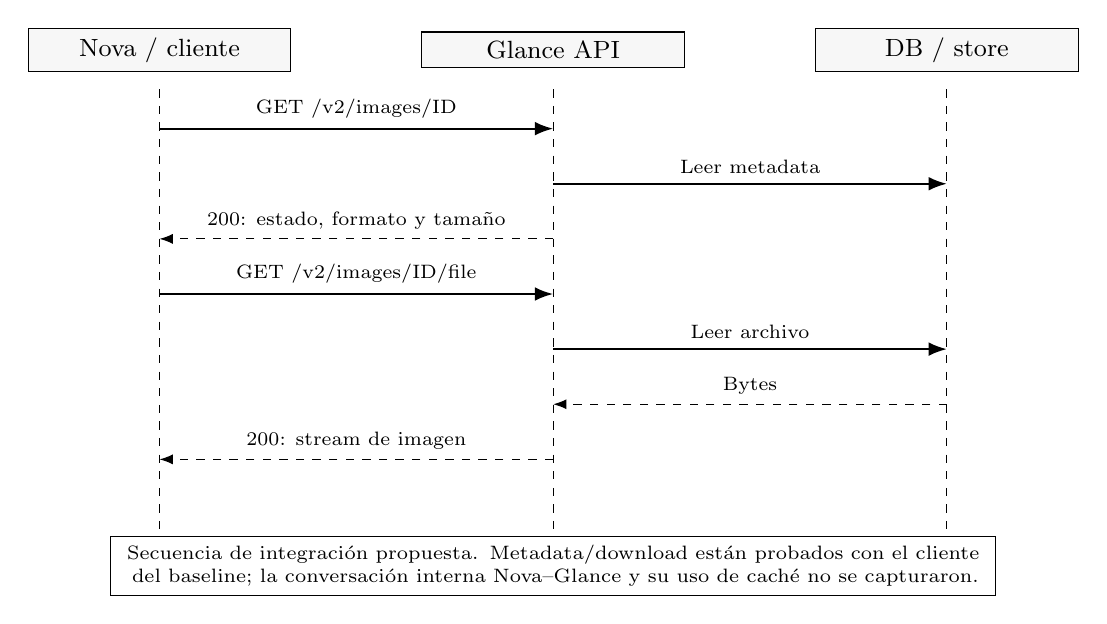
\begin{tikzpicture}[p/.style={draw,fill=black!3,text width=3.1cm,align=center,font=\small},msg/.style={-{Latex},thick},ret/.style={-{Latex},dashed},font=\scriptsize]
\node[p](nova) at (0,0){Nova / cliente};\node[p](glance) at (5,0){Glance API};\node[p](store) at (10,0){DB / store};
\foreach \x in {0,5,10}{\draw[dashed](\x,-0.5)--(\x,-6.7);}
\draw[msg](0,-1)--node[above]{GET /v2/images/ID}(5,-1);
\draw[msg](5,-1.7)--node[above]{Leer metadata}(10,-1.7);
\draw[ret](5,-2.4)--node[above]{200: estado, formato y tamaño}(0,-2.4);
\draw[msg](0,-3.1)--node[above]{GET /v2/images/ID/file}(5,-3.1);
\draw[msg](5,-3.8)--node[above]{Leer archivo}(10,-3.8);
\draw[ret](10,-4.5)--node[above]{Bytes}(5,-4.5);
\draw[ret](5,-5.2)--node[above]{200: stream de imagen}(0,-5.2);
\node[draw,align=center,text width=11cm,fill=white] at (5,-6.55){Secuencia de integración propuesta. Metadata/download están probados con el cliente del baseline; la conversación interna Nova--Glance y su uso de caché no se capturaron.};
\end{tikzpicture}
\caption{Secuencia de consumo de imagen que deberá validarse con Glance Go. Solicitudes continuas, respuestas discontinuas; la DB y el store se agrupan sólo para esta vista.}
\label{fig:sequence}
\end{figure}
\FloatBarrier

\Needspace{390pt}
\subsection{Requerimientos funcionales}
\reporttable{Requerimientos aplicables al módulo Glance.}{>{\raggedright\arraybackslash}p{1.4cm}>{\raggedright\arraybackslash}p{8.8cm}>{\raggedright\arraybackslash}p{4.8cm}}{\textbf{ID}&\textbf{Requerimiento}&\textbf{Verificación prevista}}{
RF01&OpenStack de un nodo reproducible.&Instalación y smoke test; base validada en S2.\\*
RF07&Persistencia consistente de metadata y ubicaciones.&Reinicio, fallos y reconciliación con store.\\*
RF08&Autenticación requerida por OpenStack.&Casos autorizados, 401 y 403.\\*
RF10&Registrar, listar, consultar, modificar y eliminar imágenes.&Comparación diferencial de Image API v2.\\*
RF10&Cargar/descargar bytes y mantener estados e integridad.&Comparación byte a byte/hash y pruebas de fallos.\\*
RF10&Permitir consumo de imagen por Nova.&Boot usando el reemplazo Glance.\\*
RF11&Observabilidad del módulo.&Logs saneados y diagnóstico de transferencias/errores.\\*
RF12&Automatización funcional y de carga.&Scripts versionados y dataset repetible.\\}
RF10 es el requisito específico de Glance en el Excel. Las filas separan sus criterios para hacerlos verificables sin crear nuevos IDs. RF07/RF08 y RF11/RF12 aportan capacidades transversales. La implementación Go sigue pendiente.

\subsection{Requerimientos no funcionales}
\reporttable{Atributos de calidad para el módulo Glance.}{>{\raggedright\arraybackslash}p{1.5cm}>{\raggedright\arraybackslash}p{3.5cm}>{\raggedright\arraybackslash}p{10cm}}{\textbf{ID}&\textbf{Atributo}&\textbf{Criterio}}{
RNF01&Compatibilidad&Comparar status, metadata, estados, errores, headers y efectos persistidos.\\*
RNF02&Rendimiento&Latencia de metadata y throughput de transferencia bajo cargas separadas.\\*
RNF03&Recursos&CPU y memoria en reposo, carga y transferencias de distintos tamaños.\\*
RNF04&Fiabilidad&Repeticiones, tasa de error y recuperación de cargas interrumpidas.\\*
RNF05&Reproducibilidad&Versiones, backend, configuración, comandos y dataset registrados.\\*
RNF06&Mantenibilidad&API, dominio, repositorio y store desacoplados, con pruebas.\\*
RNF07&Seguridad&Conservar auth/políticas; controlar rutas/permisos y evitar secretos en fixtures.\\}

\subsection{Arquitectura del reemplazo Go y criterios de aceptación}

\Needspace{340pt}
\begin{figure}[!ht]
\centering
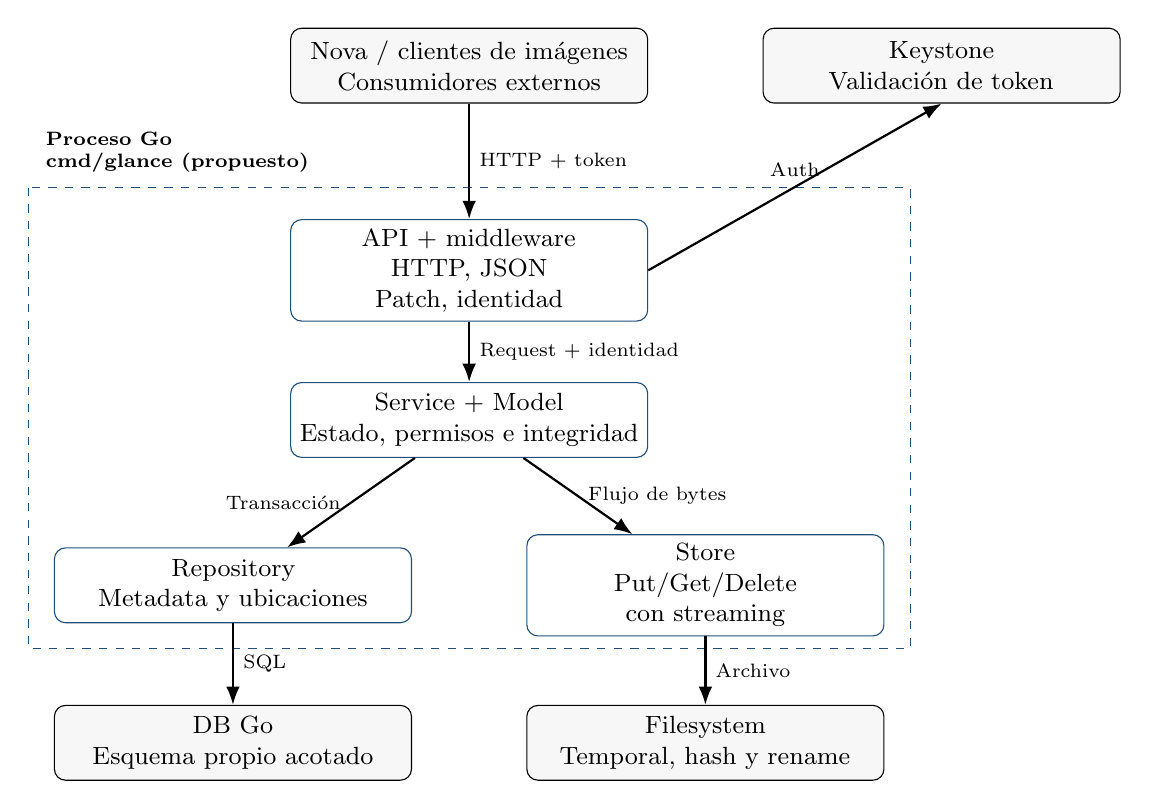
\begin{tikzpicture}[box/.style={draw=sectionblue,rounded corners,align=center,text width=4.3cm,minimum height=0.95cm,font=\small},ext/.style={box,draw=black,fill=black!3},arr/.style={-{Latex},thick}]
\node[ext](nova) at (0,2.1){Nova / clientes de imágenes\\Consumidores externos};
\node[box](api) at (0,-0.5){API + middleware\\HTTP, JSON Patch, identidad};
\node[box](svc) at (0,-2.4){Service + Model\\Estado, permisos e integridad};
\node[box](repo) at (-3,-4.5){Repository\\Metadata y ubicaciones};
\node[box](store) at (3,-4.5){Store\\Put/Get/Delete con streaming};
\node[ext](auth) at (6,2.1){Keystone\\Validación de token};
\node[ext](db) at (-3,-6.5){DB Go\\Esquema propio acotado};
\node[ext](bytes) at (3,-6.5){Filesystem\\Temporal, hash y rename};
\draw[dashed,sectionblue](-5.6,0.55) rectangle (5.6,-5.3);
\node[font=\scriptsize\bfseries,anchor=west,align=left] at (-5.5,1.0){Proceso Go\\cmd/glance (propuesto)};
\draw[arr](nova)--node[right,font=\scriptsize]{HTTP + token}(api);
\draw[arr](api)--node[right,font=\scriptsize]{Request + identidad}(svc);
\draw[arr](api.east)--node[above,font=\scriptsize]{Auth}(auth.south);
\draw[arr](svc)--node[left,font=\scriptsize]{Transacción}(repo);
\draw[arr](svc)--node[right,font=\scriptsize]{Flujo de bytes}(store);
\draw[arr](repo)--node[right,font=\scriptsize]{SQL}(db);
\draw[arr](store)--node[right,font=\scriptsize]{Archivo}(bytes);
\end{tikzpicture}
\caption{Vista de componentes del reemplazo Glance Go. El límite discontinuo delimita el proceso; DB y filesystem son dependencias separadas.}
\label{fig:go}
\end{figure}
\FloatBarrier

El ejecutable propuesto es \code{cmd/glance}. Se separan paquetes API, servicio, modelo y repositorio, con \code{glance/store} para Put/Get/Delete de bytes. Configuración, autenticación Keystone y logging son componentes compartidos. El store deberá transferir datos mediante streaming y evitar cargar el archivo completo en memoria; su comportamiento se medirá.

La aceptación requiere que original y Go superen el ciclo mínimo, que los datos descargados sean idénticos a los cargados, que estados y permisos sean compatibles y que Nova cree una instancia desde la imagen del reemplazo. Se compararán respuestas y estado con semillas equivalentes. UUID, timestamps y request IDs podrán normalizarse sin ocultar diferencias de contenido o visibilidad.

Las pruebas se organizan en unidad, contrato API, comparación diferencial, persistencia y store, integración y boot completo. Los benchmarks separarán metadata de transferencia y controlarán tamaño de imagen, concurrencia, disco, caché, warm-up y repeticiones. QEMU y el único filesystem limitan la generalización de resultados. No se presentan métricas comparativas de Go en esta etapa.


\subsection{Notación y trazabilidad de la calidad del diseño}
La vista de componentes organiza un único proceso Go, sus responsabilidades, interfaces y dependencias externas según las abstracciones del modelo C4 \cite{c4}. Los modelos ER expresan entidades y cardinalidades; las secuencias usan participantes, líneas de vida, mensajes y respuestas siguiendo la notación básica de interacción de UML \cite{uml}. Cada figura distingue sistema original, propuesta Go e intercambios todavía inferidos. Las flechas se interpretan según su leyenda; una relación del dominio no implica una FK SQL.

La compatibilidad HTTP se verificará con método, status, media type, headers y efectos, atendiendo a la semántica de HTTP y al contrato específico de OpenStack \cite{http}. Las matrices siguientes relacionan las decisiones con RF/RNF, objetivos y pruebas de aceptación. Describen prácticas de diseño y un plan de verificación; no constituyen certificación de cumplimiento de una norma ni resultados de pruebas Go.

\reporttable{Requerimientos, prácticas de diseño y verificaciones de aceptación.}{>{\raggedright\arraybackslash}p{3cm}>{\raggedright\arraybackslash}p{5.3cm}>{\raggedright\arraybackslash}p{6.4cm}}{\textbf{Requerimiento}&\textbf{Práctica / artefacto}&\textbf{Prueba o criterio}}{
RF10 / RNF01&Image API y contratos HTTP; secuencia de fig. \ref{fig:sequence}.&Comparar status, JSON Patch, media types y estados contra el original.\\*
RF07/RF10&ER y separación metadata/bytes (fig. \ref{fig:er}); ADR-02.&Persistencia, hash y tamaño; carga interrumpida y reconciliación tras reinicio.\\*
RF10 / RNF03&Store por interfaz y streaming (fig. \ref{fig:go}).&Comparar bytes y medir memoria con tamaños controlados; no asumir mejora.\\*
RF08 / RNF07&Auth Keystone; permisos y rutas filesystem; ADR-03.&401/403, propietario/visibilidad y rechazo de rutas no permitidas.\\*
RF10 / RNF06&Proceso y DB Go separados; original recuperable.&Boot de Nova con imagen del reemplazo y caché controlada.\\*
RNF05 / RF11/RF12&Versiones, logs y pruebas automatizadas.&Repetir despliegue y ciclo de imagen; guardar evidencia sin tokens ni bytes en logs.\\}
\subsection{Decisiones técnicas y alternativas}

\reporttable{Decisiones de diseño Glance y sus consecuencias.}{>{\raggedright\arraybackslash}p{1.5cm}>{\raggedright\arraybackslash}p{3.6cm}>{\raggedright\arraybackslash}p{5.2cm}>{\raggedright\arraybackslash}p{4.4cm}}{\textbf{ADR}&\textbf{Contexto y alternativas}&\textbf{Decisión y razón}&\textbf{Consecuencia / aceptación}}{
02&Metadata original, propia o proxy; store local o remoto.&Metadata propia acotada y filesystem único, coherente con el backend observado.&Validar permisos, hash, temporales y recuperación. Otro store requeriría nuevas pruebas.\\*
03&Auth: red privada, middleware Keystone o políticas completas.&Validación Keystone y políticas mínimas por operación; conservar RF08/RNF07.&Probar propietario, roles y visibilidad; no usar red privada como única autorización.\\*
Módulo&Buffer completo o transmisión por interfaz de store.&Streaming con Put/Get/Delete; separar transferencia y reglas del catálogo.&Medir CPU/RAM y throughput; controlar tamaño, caché y cargas interrumpidas.\\}

\Needspace{350pt}
\subsection{Riesgos y mitigaciones}
\reporttable{Riesgos del desarrollo Glance.}{>{\raggedright\arraybackslash}p{4.5cm}>{\raggedright\arraybackslash}p{1.5cm}>{\raggedright\arraybackslash}p{9cm}}{\textbf{Riesgo}&\textbf{Nivel}&\textbf{Mitigación}}{
Alcance de Image API demasiado amplio&Alto&Conservar ciclo mínimo y un solo backend; ampliar con evidencia de Nova.\\*
Metadata active sin bytes completos&Alto&Archivo temporal, publicación atómica y recuperación/reconciliación probada.\\*
Autorización o visibilidad incorrectas&Alto&Fixtures de propietario, roles, 401/403 y acceso permitido.\\*
Benchmark condicionado por disco/caché&Medio&Controlar estado, tamaño de archivo y carga; separar métricas.\\*
Flujo interno Nova no capturado&Medio&Captura saneada y boot controlado antes de aceptar sustitución.\\*
Dependencias secundarias variables&Medio&Registrar paquetes y congelar el entorno antes de ejecutar mediciones comparativas.\\}

\section{Planificación y backlog}
\subsection{Épicas}
Aplican las épicas del Excel vigente E1 infraestructura y entorno; E2 análisis y compatibilidad; E4 integración OpenStack; E5 pruebas y benchmarking; E6 reimplementación Glance. E3 reimplementación Placement corresponde al informe independiente de ese módulo. E7 documentación incluye B21--B24. La infraestructura común conserva su trazabilidad en ambos informes.

\Needspace{400pt}
\subsection{Backlog prioritario y estado del Sprint 2}
Los identificadores corresponden al Excel vigente \cite{plan}. El backlog preliminar del PDF de Etapa 1 fue refinado; no se utiliza su antigua numeración para asociar pruebas actuales.
\reporttable{Elementos de Sprint 2 relevantes para Glance.}{>{\raggedright\arraybackslash}p{1cm}>{\raggedright\arraybackslash}p{8.1cm}>{\raggedright\arraybackslash}p{1.2cm}>{\raggedright\arraybackslash}p{4.5cm}}{\textbf{ID}&\textbf{Elemento}&\textbf{SP}&\textbf{Estado}}{
B01&Preparar VM de laboratorio (compartido).&3&Hecho: VM auditada.\\*
B02&Instalar DevStack de un nodo (compartido).&5&Hecho: endpoints verificados.\\*
B03&Smoke tests del original (compartido).&5&Hecho: boot ACTIVE y limpieza.\\*
B19&Analizar arquitectura, Image API, auth, persistencia y flujo de Glance.&5&Hecho: especificación y baseline.\\}
La tarea específica de análisis Glance suma 5 SP; las tareas comunes, 13 SP. El Sprint 2 conjunto alcanzó 7/7 elementos y 33/33 SP al incluir B04--B06 de Placement. Esto describe aceptación de la planificación compartida, no productividad individual ni porcentaje implementado de Glance.

Las capturas están en \code{evidence/sprint2/glance/}, incluidas auditoría de backend, resultados de API y \code{image-download.sha256.txt}. El boot está en \code{evidence/sprint2/tests/boot-states.txt}; el modelo y la arquitectura se documentan en \code{docs/sprint2/}. El registro \code{infra/devstack/versions.lock} fija el código inspeccionado. La verificación \code{make sprint2-verify} aprobó las evidencias requeridas.

\subsection{Inventario de diseño y comparación con el backlog completo}
El backlog vigente contiene 26 elementos y 185 SP: 7 Hecho, 1 En progreso y 18 Pendiente. El avance global por elementos terminados es $7/26=26{,}9\%$; por puntos aceptados es $33/185=17{,}8\%$. B21 no se cuenta como terminado ni se prorratean sus puntos. Estas métricas globales se distinguen del 100\% de aceptación del Sprint 2 ($7/7$, 33/33 SP).

El conjunto de análisis y diseño central comprometido en S2 es el conjunto $D_{S2}$, formado por B04, B05, B06 y B19: 4 de 4 elementos terminados, 20 de 20 SP. En este informe, la evidencia propia del módulo se desarrolla por separado; el otro módulo aporta su expediente independiente.

Al revisar el backlog completo, B21 incluye documentación de arquitectura y decisiones como actividad continua de S3 y B16 diseña el protocolo experimental en S4. Sus estados formales siguen En progreso y Pendiente, respectivamente. Por ello, el 100\% anterior describe exclusivamente el diseño central de S2: no acredita por sí solo el cierre de todas las actividades de diseño y documentación del proyecto. Los diagramas y matrices de esta revisión amplían el soporte de B21 sin modificar el estado del Excel.


\Needspace{590pt}
\reporttable{Backlog completo: clasificación y estado formal al 2 de octubre de 2026.}{>{\raggedright\arraybackslash}p{0.9cm}>{\raggedright\arraybackslash}p{4.8cm}>{\raggedright\arraybackslash}p{3.3cm}>{\raggedright\arraybackslash}p{0.8cm}>{\raggedright\arraybackslash}p{1.3cm}>{\raggedright\arraybackslash}p{2.9cm}}{\textbf{ID}&\textbf{Elemento resumido}&\textbf{Naturaleza}&\textbf{SP}&\textbf{Sprint}&\textbf{Estado}}{
B01&Preparar VM&Entorno&3&S2&Hecho\\
B02&Instalar DevStack&Entorno&5&S2&Hecho\\
B03&Smoke tests del original&Entorno&5&S2&Hecho\\
B04&Arquitectura Placement&Diseño S2&5&S2&Hecho\\
B05&Endpoints y microversiones&Diseño S2&5&S2&Hecho\\
B06&Interacción Nova--Placement&Diseño S2&5&S2&Hecho\\
B07&Providers e inventories&Implementación&8&S3&Pendiente\\
B08&Traits y resource classes&Implementación&8&S3&Pendiente\\
B09&Allocations&Implementación&8&S3&Pendiente\\
B10&Allocation candidates&Implementación&13&S3&Pendiente\\
B11&Persistencia Placement&Implementación&8&S3&Pendiente\\
B12&Autenticación OpenStack&Implementación&8&S3&Pendiente\\
B13&Sustituir Placement&Integración&8&S4&Pendiente\\
B14&Boot con Placement Go&Integración&8&S4&Pendiente\\
B15&Suite de integración&Integración&8&S4&Pendiente\\
B16&Metodología de benchmarking&Diseño experimental&5&S4&Pendiente\\
B17&Latencia y throughput&Medición&5&S5&Pendiente\\
B18&CPU y memoria&Medición&5&S5&Pendiente\\
B19&Análisis integral Glance&Diseño S2&5&S2&Hecho\\
B20&Catálogo de metadatos Glance&Implementación&13&S4&Pendiente\\
B21&Arquitectura y decisiones (continua)&Diseño y documentación&5&S3&En progreso\\
B22&Instalación, despliegue y pruebas&Documentación&5&S4&Pendiente\\
B23&Resultados comparativos&Análisis&8&S5&Pendiente\\
B24&Informe final&Entrega&8&S5&Pendiente\\
B25&Carga/descarga Glance&Implementación&13&S4&Pendiente\\
B26&Sustitución Glance y boot Nova&Integración&8&S5&Pendiente\\}


\subsection{Repositorio, decisiones y cambios trazables}
Código, fuentes y evidencias se entregan en el \href{https://github.com/PaoloCastanon/modules-devstack-optimized}{repositorio GitHub del proyecto}. El historial Git conserva cambios con mensajes que identifican su propósito. La revisión base de los informes individuales es \code{06b6505}; las fuentes editables están en \code{docs/sprint2/reports/} y los PDF en \code{output/pdf/}. El registro de diseño se apoya en \code{design-decisions.md}, \code{go-target-architecture.md}, los contratos API y las evidencias saneadas de \code{evidence/sprint2/}.


\reporttable{Cambios de infraestructura y evidencia registrados en Git.}{>{\raggedright\arraybackslash}p{1.8cm}>{\raggedright\arraybackslash}p{5.5cm}>{\raggedright\arraybackslash}p{7.4cm}}{\textbf{Commit}&\textbf{Cambio registrado}&\textbf{Justificación y evidencia}}{
6e0ea2d&Instalación DevStack mediante Ansible.&Aprovisionamiento repetible con versión fijada; infraestructura común y scripts en infra/.\\*
b261278&Inicializar asignaciones Geneve antes de crear la red.&Corrección técnica necesaria para completar DevStack; parche versionado y posterior smoke test.\\*
6abd728&Conservar MySQL durante las ejecuciones Ansible.&Evitar que una dependencia de cliente retire el servidor; reprovisión del laboratorio.\\*
30491e9&Capturar baseline y verificaciones reales.&Servicio original, APIs, tablas, store y boot documentados en evidence/sprint2/.\\*
5052749&Actualizar el libro derivado con evidencia.&Estados Hecho de S2 sustentados; original sin modificar.\\*
203f001 /\newline 06b6505&Separar informes Placement y Glance.&Un autor y módulo por entrega; conserva evidencia común y formato institucional.\\*
6344e3f&Preservar evidencia aceptada al repetir provisión.&Evitar que una repetición sustituya las capturas ya usadas para aceptación.\\}


\Needspace{415pt}
\subsection{Refinamientos y desviaciones respecto del plan inicial}

\reporttable{Cambios del plan y justificación documental.}{>{\raggedright\arraybackslash}p{4.1cm}>{\raggedright\arraybackslash}p{5.3cm}>{\raggedright\arraybackslash}p{5.3cm}}{\textbf{Referencia inicial}&\textbf{Estado de Etapa 2}&\textbf{Justificación y efecto}}{
Backlog preliminar B01--B20 del informe de Etapa 1.&Excel vigente B01--B26; incorpora tareas técnicas y alcance Glance refinado.&Se usan los IDs del libro actual en todas las evidencias; no se equiparan automáticamente los IDs antiguos.\\*
Entorno de un nodo previsto.&VM dedicada gestionada por Terraform/libvirt y Ansible; Nova usa QEMU emulado.&Aislar el laboratorio del host y reconstruir su configuración. La emulación limita la generalización del benchmark.\\*
Reimplementación compatible por delimitar.&Placement por rutas/microversiones seleccionadas; Glance con Image API v2 y un filesystem.&El baseline y el tráfico del original acotan lo necesario. No se promete cobertura completa ni todos los stores.\\*
Persistencia del reemplazo por resolver.&Esquema propio y DB aislada; Glance separa metadata de bytes.&ADR-01/ADR-02 reducen acoplamiento al original; exigen semillas, migración y reconciliación.\\*
Informe conjunto de ambos módulos.&Dos informes individuales por instrucción de entrega.&Placement para Paolo Castañon Barrera y Glance para Juan Cardenas Uribe; las tareas comunes no se cuentan dos veces.\\*
Cronograma del libro vigente.&Se conservan S2--S5 y sus estados; B20/B25 en S4 y B26 en S5.&La preparación de fixtures en S3 no adelanta formalmente las historias Glance. No se replanificó el Excel en esta revisión.\\}


\Needspace{365pt}
\subsection{Matriz de evidencia para los criterios técnicos de Etapa 2}
La pauta del curso denomina esta etapa \textit{Diseño e Implementación Inicial}. Los tres criterios técnicos se verifican con el informe, el libro de seguimiento y el repositorio \cite{rubric}. Sus pesos originales se conservan en el cuadro; no se convierten en una nota ni en un porcentaje de logro académico.

\reporttable{Localización de evidencia para los criterios técnicos de la pauta.}{>{\raggedright\arraybackslash}p{4.2cm}>{\raggedright\arraybackslash}p{1.1cm}>{\raggedright\arraybackslash}p{9.4cm}}{\textbf{Criterio}&\textbf{Peso}&\textbf{Evidencia verificable y límite}}{
Avance en el diseño&10\%&Inventario de diseño S2 y backlog completo en esta sección. B04/B05/B06/B19: 4/4; B21 y B16 conservan estados del libro. No se afirma 100\% del diseño global.\\*
Calidad del diseño&55\%&Figuras \ref{fig:go}, \ref{fig:er} y \ref{fig:sequence}; matriz RF/RNF--práctica--prueba; contratos y ADR del módulo. Diferencia explícita entre diseño y validación Go posterior.\\*
Documentación del proyecto&15\%&Fuentes y PDF, URL Git, decisiones con alternativas/consecuencias, registro de commits y refinamientos del plan. Evidencia de pruebas originales y archivos de reproducción.\\}

\Needspace{240pt}
\subsection{Plan por sprints e hitos}
\reporttable{Hitos del módulo Glance.}{>{\raggedright\arraybackslash}p{3.2cm}>{\raggedright\arraybackslash}p{2.4cm}>{\raggedright\arraybackslash}p{9.4cm}}{\textbf{Periodo}&\textbf{Hito}&\textbf{Resultado esperado}}{
Hasta 04-09&Etapa 1&Problema, objetivos y alcance mínimo de imágenes.\\*
05-09 a 02-10&Etapa 2 / S2&Arquitectura, API, estados, backend y baseline original.\\*
03-10 a 30-10&Etapa 3 / S3&Hito común de 50\% del proyecto; preparar esqueleto, contratos y fixtures de Glance. B20/B25 permanecen en S4.\\*
31-10 a 20-11&Cierre / S4&Implementar catálogo mínimo (B20) y carga/descarga (B25); integrar auth y recuperación. Preparar B26.\\*
21-11 a 04-12&Evaluación / S5&Sustituir Glance y validar boot con Nova (B26); comparar metadata/transferencia y preparar conclusiones.\\}

\Needspace{320pt}
\section{Conclusiones de la Etapa 2}
El cierre del diseño central de S2 se sustenta en cuatro elementos terminados y en su comparación con los 26 elementos del backlog. Esta revisión incorpora vistas del reemplazo Go, modelo ER, secuencia, decisiones y trazabilidad de calidad. B21 y B16 conservan su estado formal; no se confunde la aceptación del Sprint 2 con el cierre de todo el diseño o con la implementación del reemplazo.

Glance quedó delimitado a un ciclo mínimo de Image API v2 y un store filesystem. La evidencia original confirma registro, consulta, modificación, carga, descarga íntegra y eliminación, junto con el rechazo sin token. El smoke test de OpenStack alcanzó ACTIVE desde CirrOS.

OE1 y OE2 se cumplen para el alcance de Sprint 2. La integración específica del reemplazo Go, las políticas adicionales, los estados de fallo y los benchmarks permanecen como trabajo posterior. No se infiere equivalencia completa a partir del ciclo principal ni se atribuye a Go una mejora aún no medida.

El siguiente paso es implementar metadatos y persistencia, desarrollar el store con streaming y recuperación, y comparar cada operación con la línea base. La captura del flujo Nova--Glance completará la evidencia de integración a medida que avance el desarrollo.

\Needspace{280pt}
\begingroup\small
\phantomsection\addcontentsline{toc}{section}{Referencias}
\begin{thebibliography}{9}
\bibitem{glanceoverview} OpenStack. \textit{Image service overview -- Glance}. Referencia utilizada en el informe de Etapa 1. \url{https://docs.openstack.org/glance/latest/install/get-started.html}.
\bibitem{glanceapi} OpenStack. \textit{Image Service API v2}. \url{https://docs.openstack.org/api-ref/image/v2/}.
\bibitem{devstack} OpenStack. \textit{DevStack Documentation}. \url{https://docs.openstack.org/devstack/latest/}.
\bibitem{repo} Proyecto \textit{modules-devstack-optimized}. Documentación y evidencias Sprint 2, capturadas el 2 de octubre de 2026. Directorios \code{docs/sprint2/}, \code{evidence/sprint2/} e \code{infra/}; registro de evidencia y matriz final de trazabilidad.
\bibitem{plan} \textit{Planificacion\_Trabajo\_Titulo\_OpenStack\_Placement\_Glance.xlsx} y copia de seguimiento Sprint 2. Hojas Objetivos\_SMART, Requerimientos, Backlog, Trazabilidad y Sprints. La copia original se mantiene inalterada.

\bibitem{c4} Simon Brown. \textit{C4 model: Component diagram}. Vista de componentes de un contenedor y sus dependencias. \url{https://c4model.com/diagrams/component}. Consultado el 2 de octubre de 2026.
\bibitem{uml} Object Management Group. \textit{Unified Modeling Language, versión 2.5.1}. \url{https://www.omg.org/spec/UML/2.5.1}. Referencia de notación de interacción; consultado el 2 de octubre de 2026.
\bibitem{http} IETF. \textit{RFC 9110: HTTP Semantics}. Junio de 2022. \url{https://www.rfc-editor.org/rfc/rfc9110.html}. Consultado el 2 de octubre de 2026.
\bibitem{rubric} Universidad Católica de Temuco. \textit{Pauta y rúbrica de evaluación del curso de Trabajo de Título (INFO-1197)}. 17 de agosto de 2026. Etapa 2, página 3. Documento proporcionado para esta revisión.
\end{thebibliography}
\endgroup
\end{document}
